%
% jordan-ungleichung.tex
%
% (c) 2026 Damien Flury, OST Ostschweizer Fachhochschule
%
\begin{figure}
\centering
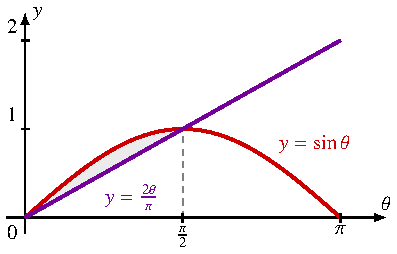
\includegraphics{papers/hauptwert/images/jordan-ungleichung.pdf}
\caption{Auf dem Intervall $[0,\frac{\pi}{2}]$ verläuft der Sinusbogen
oberhalb seiner Sehne, es gilt also $\sin\theta \ge \frac{2\theta}{\pi}$.
Beide Kurven treffen sich in den Endpunkten $0$ und $\frac{\pi}{2}$.
\label{hauptwert:figure:jordan-ungleichung}}
\end{figure}
